%----------------------------------------------------------------------------------------
% PACKAGES AND OTHER DOCUMENT CONFIGURATIONS
%----------------------------------------------------------------------------------------

\documentclass{article}

\usepackage{fancyhdr} % Required for custom headers
\usepackage{lastpage} % Required to determine the last page for the footer
\usepackage{extramarks} % Required for headers and footers
\usepackage[usenames,dvipsnames]{color} % Required for custom colors
\usepackage{graphicx} % Required to insert images
\usepackage{listings} % Required for insertion of code
\usepackage{lipsum} % Used for inserting dummy 'Lorem ipsum' text into the template
\usepackage[utf8]{inputenc}
\usepackage[T1]{fontenc}
\usepackage{stmaryrd}
\usepackage[frenchb]{babel}
\usepackage{amsmath}
\usepackage{amsthm}
\usepackage{amsfonts}

% Margins
\topmargin=-0.45in
\evensidemargin=0in
\oddsidemargin=0in
\textwidth=6.5in
\textheight=9.0in
\headsep=0.25in

\linespread{1.1} % Line spacing

% Set up the header and footer
\pagestyle{fancy}
\lhead{\hmwkAuthorName} % Top left header
\chead{\hmwkTitle} % Top center head
\rhead{\firstxmark} % Top right header
\lfoot{\lastxmark} % Bottom left footer
\cfoot{} % Bottom center footer
\rfoot{Page\ \thepage\ sur\ \protect\pageref{LastPage}} % Bottom right footer
\renewcommand\headrulewidth{0.4pt} % Size of the header rule
\renewcommand\footrulewidth{0.4pt} % Size of the footer rule

\setlength\parindent{0pt} % Removes all indentation from paragraphs

%----------------------------------------------------------------------------------------
% CODE INCLUSION CONFIGURATION
%----------------------------------------------------------------------------------------

\lstloadlanguages{C} % Load Perl syntax for listings, for a list of other languages supported see: ftp://ftp.tex.ac.uk/tex-archive/macros/latex/contrib/listings/listings.pdf
\lstset{texcl=true, columns=flexible,basicstyle=\small\ttfamily}

\lstdefinestyle{ccode}{language=C, % Use Perl in this example
        frame=single, % Single frame around code
        basicstyle=\small\ttfamily, % Use small true type font
        keywordstyle=[1]\color{Blue}, % Perl functions bold and blue
        keywordstyle=[2]\color{Green}, % Perl function arguments purple
        keywordstyle=[3]\color{Blue}, % Custom functions underlined and blue
        identifierstyle=, % Nothing special about identifiers
        commentstyle=\small\color{Brown}, % Comments small dark green courier font
        stringstyle=\color{OliveGreen}, % Strings are purple
        showstringspaces=false, % Don't put marks in string spaces
        tabsize=5, % 2 spaces per tab
        %
        % Put standard Perl functions not included in the default language here
        morekeywords={f, sequantial_computation, parallel_computation, printf},
        morecomment=[l][\color{Brown}]{...}, % Line continuation (...) like blue comment
        numbers=left, % Line numbers on left
        firstnumber=1, % Line numbers start with line 1
        numberstyle=\tiny\color{Blue}, % Line numbers are blue and small
        stepnumber=5, % Line numbers go in steps of 5
        texcl=true,
        columns=flexible
}

%----------------------------------------------------------------------------------------
% NAME AND CLASS SECTION
%----------------------------------------------------------------------------------------

\newcommand{\hmwkTitle}{Calcul de $\pi$} % Assignment title
\newcommand{\hmwkClass}{High Performance Computing} % Course/class
\newcommand{\hmwkClassInstructor}{F. Magoules} % Teacher/lecturer
\newcommand{\hmwkAuthorName}{Plessia Stanislas} % Your name

%----------------------------------------------------------------------------------------
% TITLE PAGE
%----------------------------------------------------------------------------------------

\title{
\LARGE{\textbf{\hmwkClass}}\\
\vspace{0.5in}
\large{\textbf{\hmwkTitle}}
\vspace{3in}
}

\author{\textbf{\hmwkAuthorName}}
\date{Février 2018} % Insert date here if you want it to appear below your name

%----------------------------------------------------------------------------------------

\begin{document}

\maketitle

%----------------------------------------------------------------------------------------
% TABLE OF CONTENTS
%----------------------------------------------------------------------------------------

%\setcounter{tocdepth}{1} % Uncomment this line if you don't want subsections listed in the ToC

\newpage
\tableofcontents
\newpage

%----------------------------------------------------------------------------------------
% PROBLEM 1
%----------------------------------------------------------------------------------------

% To have just one problem per page, simply put a \clearpage after each problem

\section{Analyse}

\subsection{Définition du problème}

On veut calculer une valeur approximative de $\pi$. Pour cela, nous allons utiliser le fait que $arctan(1) = \dfrac{\pi}{4}$\\

Pour calculer cette valeur, nous allons effetuer le calcul suivant :\\

\[
   \pi = 4(arctan(1) - arctan(0)) = 4\int_0^1 \dfrac{d(arctan(x))}{dx}dx =  4\int_0^1 \dfrac{1}{1 + x^2} dx
\]\\


Ainsi en calculant une intégrale il est possible d'avoir une valeur approchée de $\pi$.
Le calcul d'intégrale est un classique algorithmique, nous allons utiliser la méthode des trapèzes:\\

On subdivise le domaine de l'intégrale $[a,b]$ en $n$ segments $[a_i, a_{i+1}]_{i\in\llbracket0,n-1\rrbracket}$
avec $a_0 = a$, $a_{n} = b$,  soit :\\

\[
a_i = a + i \cdot \dfrac{b-a}{n} \mbox{ et } \int_a^b f(x)dx = \sum_{i=0}^{n-1}\left(\int_{a_i}^{a_{i+1}}f(x)dx\right)
\]\\

Chaque petite intégrale est ensuite approchée par l'aire du trapèze de sommet $(a_i, a_{i+1}, f(a_{i+1}), f(a_i))$ soit :\\

\[
\int_{a_i}^{a_{i+1}}f(x)dx \approx \left(a_{i+1}-a_i)\right)\cdot\dfrac{f(a_{i+1})+f({a_i})}{2} = \dfrac{b-a}{n}\cdot\dfrac{f(a_{i+1})+f({a_i})}{2}
\]

Donc : 

\begin{align*}
    \int_{a}^{b}f(x)dx &\approx \sum_{i=0}^{n-1}\left(a_{i+1}-a_i)\right)\cdot\dfrac{f(a_{i+1})+f({a_i})}{2} \\
    &= \dfrac{b-a}{n}\cdot\sum_{i=0}^{n-1}\dfrac{f(a_{i+1})+f({a_i})}{2}\\
    &= \dfrac{b-a}{n}\cdot\left(\sum_{i=1}^{n-1}f(a_{i}) + \dfrac{f(a) + f(b)}{2}\right)
\end{align*}

D'où le code:

\begin{lstlisting}[style=ccode, morekeywords={f}]
double trapeze(double a, double b, int n){
  double h = (b - a)/n;
  double integral = (f(a) + f(b))/2;
  for( int k = 1; k < n; k++){
    integral += f(a + k * h);
  }
  integral *= h;
  printf("%lf, %lf, %lf, %d\n", integral, a, b, n);
  return integral;
}
\end{lstlisting}

\section{Implémentation}
\subsection{Parallélisation}

Nous devons à présent paralléliser ce programme.
La boucle ne semble présenter aucune dépendance et peut donc être facilement parallélisée.\\

Les paramètres du problèmes sont alors : 
\begin{itemize}
    \item Le nombre de subdivision du domaine intégral $n$
    \item Le nombre de processeur qui vont faire le calcul $p$
\end{itemize}

L'objectif est alors de découper l'intégrale en $p$ sous intégrales qui seront chacune calculée dans un processeur.
Le résultat de chaque sous intégrale seraenvoyée au processeur \texttt{root} qui ajoutera les résultats pour afficher l'initégrale globale.\\

\begin{lstlisting}[style=ccode, morekeywords={f, MPI_Recv, MPI_Send, trapeze_sequential}]
int main(int argc, char* argv[]){
  double a = 0, b = 1;
  int n = 24000; // default subdivision value
  double integral;
  if ( argc > 1){
    n = atoi(argv[1]);
  }
  double pas = (b-a)/n;

  int rank, size;
  MPI_Init(&argc, &argv);               // starts MPI
  MPI_Comm_rank(MPI_COMM_WORLD, &rank); // get current process id
  MPI_Comm_size(MPI_COMM_WORLD, &size); // get number of processes

  switch(rank){
    case 0:
      integral = trapeze(a, a + pas * n / size, n / size );
      double int_from_sub_proc;

      for( int k = 1; k < size; k++){
        printf("Receving data from proc %d\n", k);
        MPI_Recv(&int_from_sub_proc, 1, MPI_DOUBLE, k, 0, MPI_COMM_WORLD, MPI_STATUS_IGNORE);
        integral += int_from_sub_proc;
      }
      printf("Integral value : %lf, with error %.3e\n", integral, M_PI - integral);
    break;
    default:
      printf("Calculating process %d\n", rank);
      double loca = a + rank * pas * n / size;
      double locb = loca + pas * n / size;

      double inte = trapeze(loca, locb, n / size );
      MPI_Send(&inte, 1, MPI_DOUBLE, 0, 0,  MPI_COMM_WORLD);
    break;
  }

  MPI_Finalize();
}
\end{lstlisting}

\newpage

\section{Résultats}

\subsection{Vitesse d'exécution}

Essayons d'estimer le temps gagné en passant le calcul sur plusieurs processus.\\

Les valeurs de n testées sont : $24\cdot10^k , k \in \llbracket 0,6\rrbracket$\\

Pour $n<10^8$, la différence n'est pas sensible et le processeur n'a pas le temps de monter à 100\% d'utilisation.
De façon étonnante, Lecomportement n'est pas linéaire par rapport au nombre de processeurs, et semble perturbant pour certaines valeurs de $p$.\\

J'ai fais l'experience sur un processeur \texttt{Intel(R) Core(TM) i7-6700HQ CPU @ 2.60GHz} qui dispose de 4 coeurs physiques et de 8 coeurs logiques. 

\begin{figure}[h]
    \centering
    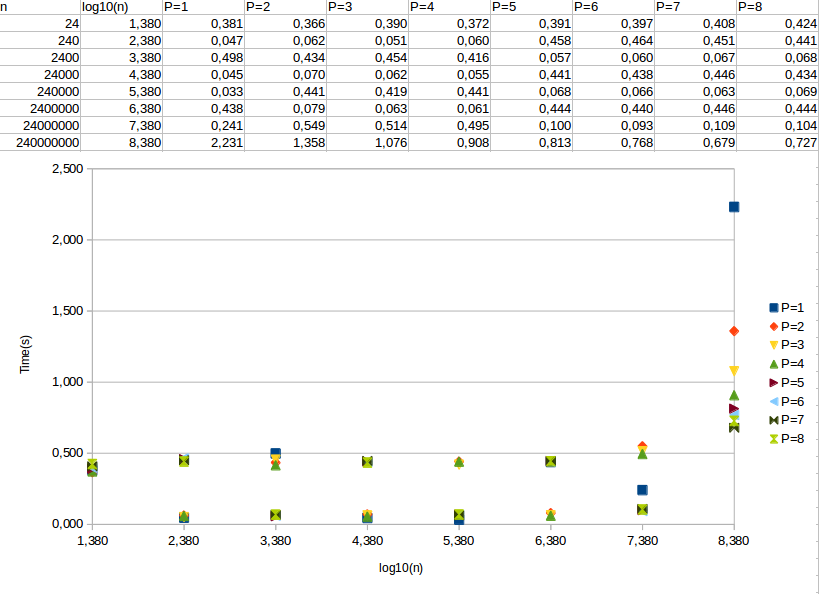
\includegraphics[width=300pt]{perf_pi.png}
    \caption{Performance du programme en fonction de $n$ et de $p$}
\end{figure}

\subsection{Précision}

Pour comparer les précisions, j'utilise la constante $\pi$ de \textbf{math.h}.
On prend soin de garder $n$ divisible par $k$ pour que les processus aient la même charge de travail et qu'ils aient chacun les même erreurs.\\

Le nombre de processus affecte très peu la précision. Je suppose que l'on voie des différences dûes aux processus pour $n=240000$, puis l'on atteint les limites de précision des \lstinline[style=ccode]|double|. On remarque que à chaque pas (10 fois plus de trapèzes), la précision est multipliée par 100, ce qui est cohérent avec la majoration de l'erreur de cet algorithme:\\

\[
\left|\int_{a}^{b}f(x)\mathrm{d}x -T_n \right| \leq \dfrac{M(b-a)^3}{12n^2}
\]

avec $T_n$ l'approximation avec $n$ trapèzes, $M$ constante dépendant de $f$ supposée de classe $\mathcal{C}^2$ sur $[a,b]$.
\end{document}